% SPDX-License-Identifier: CC-BY-4.0
% SPDX-FileCopyrightText: 2026 Dan C. Hsu and Luke Lu
% Repository rendering of the GRACE paper figure: https://arxiv.org/abs/2607.09175
\documentclass[tikz,border=3pt]{standalone}
\usepackage{xcolor}
\usetikzlibrary{arrows.meta}

\definecolor{rsupports}{HTML}{1A1A1A}
\definecolor{rrefines}{HTML}{8B4513}
\definecolor{rsequence}{HTML}{2C5F5F}
\newcommand{\typename}[1]{\texttt{#1}}

\begin{document}
\pagecolor{white}
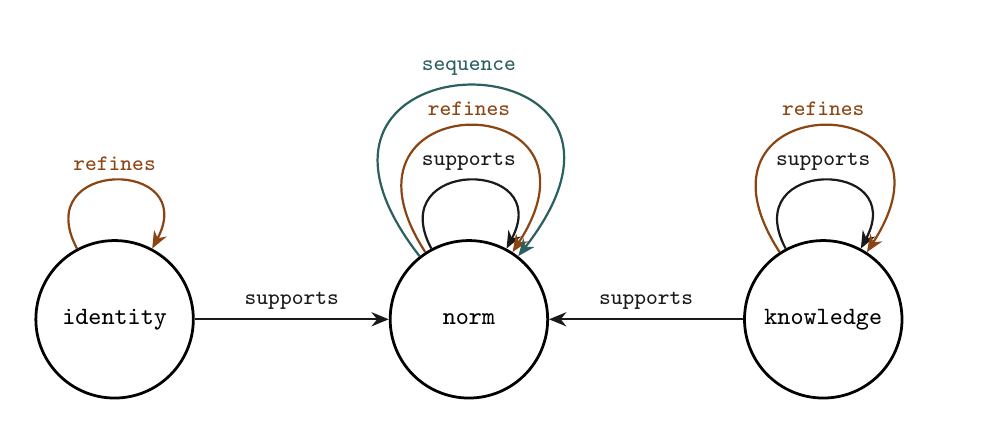
\begin{tikzpicture}[
  >={Stealth[length=2.2mm, width=1.8mm]},
  type/.style={
    circle, draw=black, line width=1pt,
    minimum size=2cm, inner sep=0pt,
    font=\small
  },
  rel/.style={->, line width=0.8pt},
  lbl/.style={font=\footnotesize},
]
  \node[type] (identity)  at (-4.5, 0) {\typename{identity}};
  \node[type] (norm)      at (0, 0)    {\typename{norm}};
  \node[type] (knowledge) at (4.5, 0)  {\typename{knowledge}};

  \draw[rel, color=rsupports] (identity) --
    node[lbl, above, color=rsupports] {\typename{supports}} (norm);
  \draw[rel, color=rsupports] (knowledge) --
    node[lbl, above, color=rsupports] {\typename{supports}} (norm);

  \draw[rel, color=rrefines] (identity)
    to[out=118, in=62, looseness=3.5]
    node[lbl, above, color=rrefines] {\typename{refines}} (identity);

  \draw[rel, color=rsupports] (norm)
    to[out=118, in=62, looseness=3.5]
    node[lbl, above, color=rsupports] {\typename{supports}} (norm);
  \draw[rel, color=rrefines] (norm)
    to[out=123, in=57, looseness=5.9]
    node[lbl, above, color=rrefines] {\typename{refines}} (norm);
  \draw[rel, color=rsequence] (norm)
    to[out=128, in=52, looseness=7.5]
    node[lbl, above, color=rsequence] {\typename{sequence}} (norm);

  \draw[rel, color=rsupports] (knowledge)
    to[out=118, in=62, looseness=3.5]
    node[lbl, above, color=rsupports] {\typename{supports}} (knowledge);
  \draw[rel, color=rrefines] (knowledge)
    to[out=123, in=57, looseness=5.9]
    node[lbl, above, color=rrefines] {\typename{refines}} (knowledge);
\end{tikzpicture}
\end{document}
